\documentclass{beamer}

% set font
\usepackage{fontspec}
\setmainfont{Noto Serif CJK SC}
\setsansfont{Noto Sans CJK SC}
\setmonofont{Noto Sans Mono CJK SC}

\usepackage{minted}

\usepackage{ctex, hyperref}
\usepackage[T1]{fontenc}

% other packages
\usepackage{latexsym,amsmath,xcolor,multicol,booktabs,calligra}
\usepackage{graphicx,pstricks,listings,stackengine}

\title{操作系统支持矩阵国际化与自动翻译应用}
\subtitle{基于 GPT 模型的自动国际化生成}
\institute{测试小队}
\author{孙齐}
\date{2024 年 7 月 3 日}
\usepackage{Beamer}

% defs
\def\cmd#1{\texttt{\color{red}\footnotesize $\backslash$#1}}
\def\env#1{\texttt{\color{blue}\footnotesize #1}}
\definecolor{deepblue}{rgb}{0,0,0.5}
\definecolor{deepred}{rgb}{0.6,0,0}
\definecolor{deepgreen}{rgb}{0,0.5,0}
\definecolor{halfgray}{gray}{0.55}

\lstset{
    basicstyle=\ttfamily\small,
    keywordstyle=\bfseries\color{deepblue},
    emphstyle=\ttfamily\color{deepred},    % Custom highlighting style
    stringstyle=\color{deepgreen},
    numbers=left,
    numberstyle=\small\color{halfgray},
    rulesepcolor=\color{red!20!green!20!blue!20},
    frame=shadowbox,
}


\begin{document}

\begin{frame}
    \titlepage
\end{frame}

\begin{frame}
    \tableofcontents[sectionstyle=show,subsectionstyle=show/shaded/hide,subsubsectionstyle=show/shaded/hide]
\end{frame}

\section{Self}

\begin{frame}{Self}
    \begin{itemize}
        \item Github: \href{\#wychlw}{github.com/wychlw}
        \newline
        \item Email: lingwang\#wcysite.com
        \newline
        % \item Refer as 泠/凛 in most cases
    \end{itemize}
\end{frame}

\section{Support Matrix}

\begin{frame}{Support Matrix}
    \begin{itemize}
        \item Mainstream operating systems $\times$ Mainstream RISC-V development boards
        \item Installation guide with test results for each combination
        \item \url{ruyisdk.org/supported}
    \end{itemize}
    \begin{figure}
        \centering
            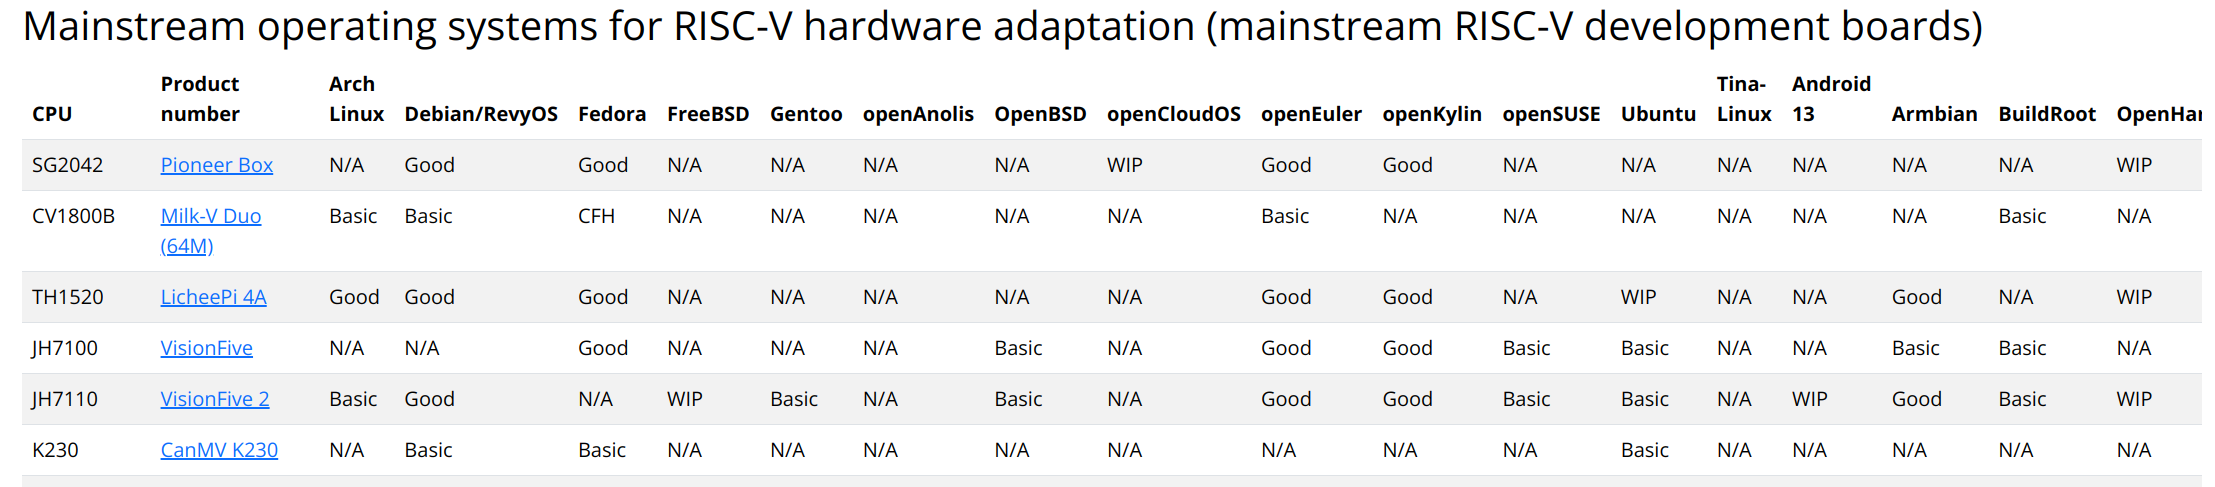
\includegraphics[width=\textwidth]{pic/matrix.png}
    \end{figure}
\end{frame}

\begin{frame}{Support Matrix}
    \begin{itemize}
        \item Check compatibility
        \item All guides in one place
        \item Provide files and scripts
    \end{itemize}
    \begin{figure}
        \centering
            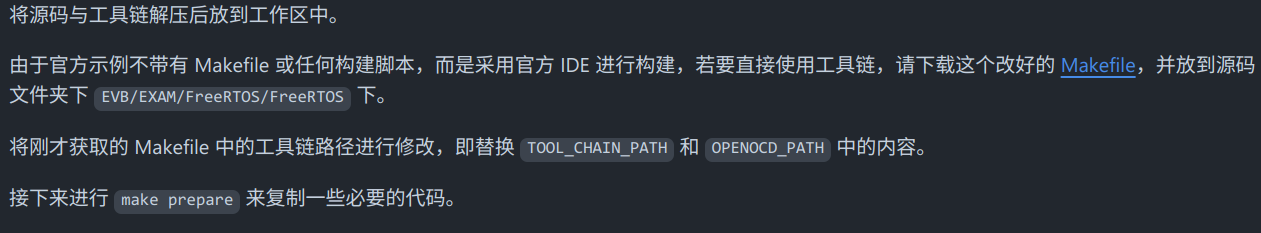
\includegraphics[width=\textwidth]{pic/make_doc.png}
    \end{figure}
\end{frame}

\begin{frame}{Support Matrix}
    \begin{itemize}
        \item Report and fix error
    \end{itemize}
    \begin{figure}
        \centering
            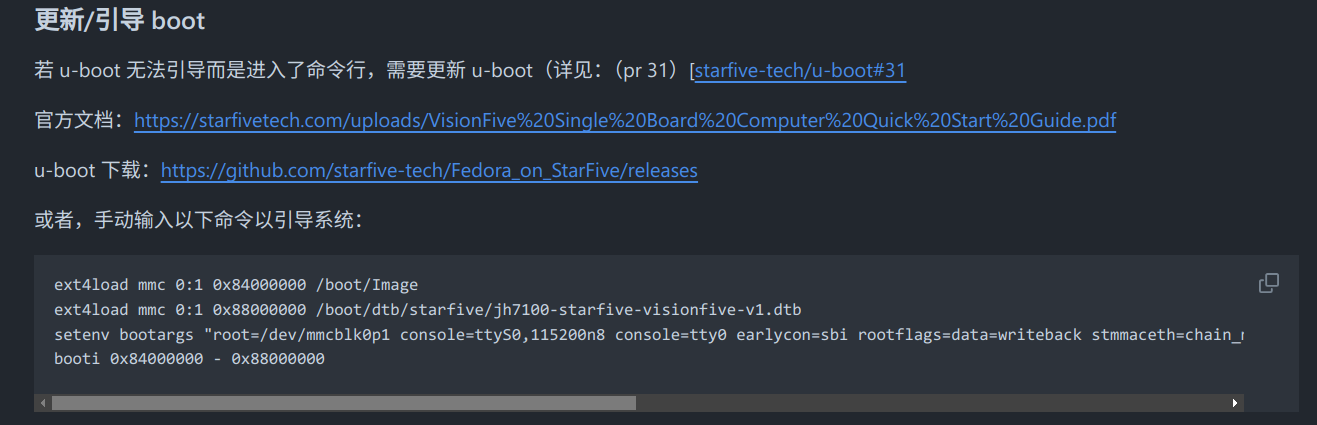
\includegraphics[width=\textwidth]{pic/prob.png}
    \end{figure}
\end{frame}

\begin{frame}{Internationalization And Problems}
    \begin{itemize}
        \item 50 development boards now with approximately 3-4 operating system each \newline
        actually: 219 reports in total
        \item Huge amount of file to be translated, need to consider human mistakes
        \item Have some kind of similarity between the reports, but lots of variations
        \item With technical terms and context
    \end{itemize}
\end{frame}

\section{How to: Use GPT}

\begin{frame}{Use GPT API}
    \begin{itemize}
        \item Basically just like in the web (no finetuning)
        \item docs: \url{platform.openai.com/docs/overview}
        \item Lots of usage: embedding, vision tts etc.
        \newline Only consider text generation
    \end{itemize}
\end{frame}

\begin{frame}{Roles}
    Three roles when talk with GPT:
    \begin{itemize}
        \item System: Model Instructions
        \item Assisstant: Model Output
        \item User: Conversation Input
    \end{itemize}
    System seems having more priority. \\
    Context is important in translation, seperate Assisstant and User having some benefits. \\
    \bigskip
    (Though in other task, impact on different roles may be vary)
\end{frame}

\begin{frame}{Parameters}
    Model have some parameters:
    \begin{itemize}
        \item temperature : ramdomness
        \item max\_token : max context length(4095 in 3.5 and 4o)
        \item top\_p : creativity (sometimes opposite to accuracy)
        \item frequency\_penalty : no repeat(generally no need to set)
        \item presence\_penalty : no same token(generally no need to set)
    \end{itemize}
\end{frame}

\begin{frame}[fragile]{Usage}
    With RESTful API (or use predefined SDK)
    \begin{minted}[
        linenos
    ]{python3}
from openai import OpenAI
client = OpenAI()

response = client.chat.completions.create(
    model="gpt-4o",
    messages=[],
    temperature=1,
    max_tokens=256,
    top_p=1,
    frequency_penalty=0,
    presence_penalty=0
)
    \end{minted}
\end{frame}

\begin{frame}[fragile]{Usage}
    Results are in JSON format, content in: \\
    \mintinline{python3}| response.choices[0].message.content |

    If out of token, \\
    \mintinline{python3}| response.choices[0].finish_reason |
    will be \mintinline{python3}| "length" |
    (continue with no new things add to message)
\end{frame}

\section{report-i18n}

\begin{frame}{Ideas of Using LLMs}
    \begin{itemize}
        \item Good quality <-> Traditional doc translation service
        \item Fast and cheap <-> Professional translator
    \end{itemize}
    \bigskip
    \bigskip
    \bigskip
    \bigskip
    \bigskip
\end{frame}

\begin{frame}{Limitation}
    \begin{itemize}
        \item Good quality <-> Traditional doc translation service
        \item Fast and cheap <-> Professional translator
    \end{itemize}
    \bigskip
    But need to pay attention\dots
    \begin{itemize}
        \item Hallucinations
        \item Secretly change minor details
        \item Manual review is still needed
    \end{itemize}
\end{frame}

\begin{frame}{Auto Translation With OpenAI GPT}
    \begin{itemize}
        \item Proj: \url{github.com/wychlw/report-i18n}
        \item Support 3.5 and 4o ( Balance between quality and price )
        \item -- Specialized for test report translation, may need to be adjusted for other purposes
    \end{itemize}
\end{frame}

\begin{frame}{Report i18n}
    \begin{itemize}
        \item Automaticlly translate docs into all target languages
        \item \mintinline{text}|\%s/README.md/README_(lang).md/| , with link changed inside
        \item Will extract everyting in codeblock and not translate them
        \item Will not translate (mostly) URLs
    \end{itemize}
\end{frame}

\begin{frame}{Usage}
    \begin{itemize}
        \item Tweaked model parameters included
        \item Config:
        \begin{itemize}
            \item env.py : API\_KEY and API\_URL 
            \newline OpenAI official and FREE API provided by GPT\_API\_free
            \item conf.py : Config lang and (part of) promote
        \end{itemize}
    \end{itemize}
\end{frame}

\begin{frame}{Usage: conf.py}
    \begin{itemize}
        \item max\_length : Max length for each iteration, generally token size if logogram else $\{3, 4\} * token size$
        \item target\_lang/tips\_translated\_by\_chatgpt : Language to translate to and the tips
        \item model: 4o if logogram to ideogram (or vise versa), else 3.5
        \item template: !important
        \newline eg: 测试成功 -> Test Passed | Test Successful | Test Succeed | Successful Test...
        \newline To regulate general structure of the translation.
    \end{itemize}
\end{frame}

\begin{frame}{Usage: Marker and CI}
    Marker is used to change default behavior (will be removed automatically):
    \begin{itemize}
        \item \mintinline{python3}|r"\[translate\]"| : Force re-translate
        \item \mintinline{python3}|r"\[update\]"| : Force update translation
        \item \mintinline{python3}|r"\[skip_lang\[(.*?)\]\]"| : Skip translate language
        \item Any other good ideas?
    \end{itemize}
    A template for CI, automatically translate and push the repo. (Notice the potential API leak)
\end{frame}

\section{Demo}

\begin{frame}{Demo: report-i18n}
    Let's now try translating a report to French? \\
    (Hopefully the network is good enough)
\end{frame}

\section{Chat Any where}

\begin{frame}{Chat Any where}
    \begin{itemize}
        \item \url{github.com/chatanywhere/GPT_API_free}
        \item Provide free API for GPT-3.5 
        \item Simply authorize it using github account to get a free key
        \item Set the API\_URL in env.py to \mintinline{text}| https://api.chatanywhere.tech/v1 |
    \end{itemize}
    \begin{figure}
        \centering
            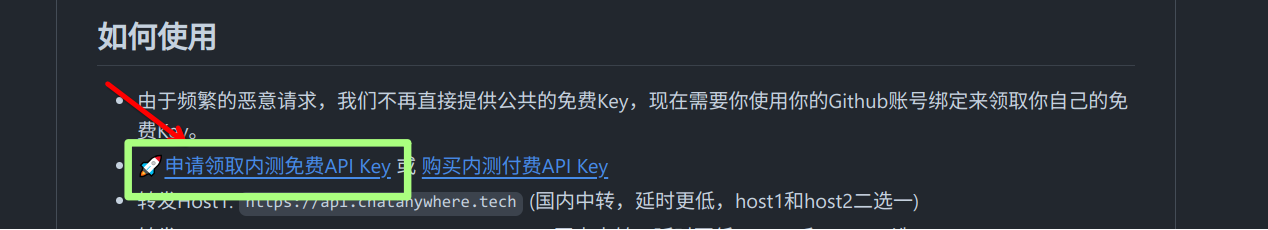
\includegraphics[width=\textwidth]{pic/get_free.png}
        \centering
            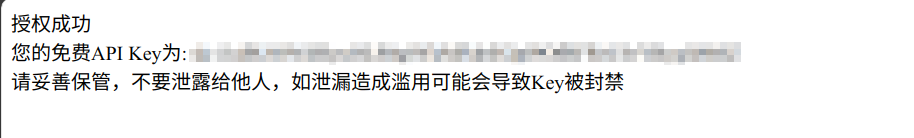
\includegraphics[width=\textwidth]{pic/free_api.png}
    \end{figure}
\end{frame}

\begin{frame}
    \begin{center}
        {\Huge Thanks for your listening!}
    \end{center}
\end{frame}

\end{document}